\documentclass{article}
\usepackage{amsmath}
\usepackage{amsthm}
\usepackage{amssymb}
\usepackage{enumerate}
\usepackage{graphicx}
\usepackage{tikz}
\usepackage{pgfplots}
\usetikzlibrary{fillbetween}
\usepgfplotslibrary{fillbetween}

\makeatletter
\newcommand{\pgfplotsdrawaxis}{\pgfplots@draw@axis}
\makeatother
\pgfplotsset{only axis on top/.style={axis on top=false, after end axis/.code={
             \pgfplotsset{axis line style=opaque, ticklabel style=opaque, tick style=opaque,
                          grid=none}\pgfplotsdrawaxis}}}

\newcommand{\drawge}{-- (rel axis cs:1,0) -- (rel axis cs:1,1) -- (rel axis cs:0,1) \closedcycle}
\newcommand{\drawle}{-- (rel axis cs:1,1) -- (rel axis cs:1,0) -- (rel axis cs:0,0) \closedcycle}

\begin{document}
    \title{Exercise 14.1}
    \author{Wang Yue from CS Elite Class}
    \date{\today}
    \maketitle

    \subsection*{11. }

    \begin{enumerate}[(a)]
        \item $f(1, 1, 1) = \sqrt 1 +\sqrt 1 +\sqrt 1 + \ln (4 - 1 - 1 - 1) = 3$
        \item 
        $\because f(x, y, z) = \sqrt x + \sqrt y + \sqrt z - \ln(4 - x - y - z)$ is defined as

        $$\left\{ \begin{array}{ll} x \geq 0 \\ y \geq 0 \\ z \geq 0 \\ 4 - x - y - z > 0 \end{array}\right.$$

        $\therefore$ The domain of $f$ is $$\{  (x, y, z) | 4 -x - y - z > 0 \textrm{ and } x \geq 0 \textrm{ and } y \geq 0 \textrm{ and } z \geq 0\}$$
    \end{enumerate}

    \subsection*{15. }
    $\because f(x, y) = \ln(9 - x^2 - 9y^2)$ is defined as $$9 - x^2 - 9y^2 > 0\qquad \textrm{or} \qquad \frac{x^2}{9} + y^2 < 1$$

    $\therefore$ The domain of $f$ is $$\{ (x, y) | \frac{x^2}{9} + y^2 < 1 \}$$

    and the graph of $D(f)$ is illustrated below.

    % \begin{figure}[htpb] 
    %     \centering 
    %     \label{fig:p3:c1} 
    %     \begin{tikzpicture} 
    %         \begin{axis}[only axis on top,
    %             axis line style=very thick, 
    %             axis x line=middle, 
    %             axis y line=middle, 
    %             ymin=-3,ymax=3,xmin=-3,xmax=3, 
    %             xlabel=$x$, ylabel=$y$,grid=major 
    %         ] 
    %             \draw [domain=-3:3, samples=200] plot({\x}, {sqrt(1-\x*\x/9)});
    %             % \addplot [draw=none, pattern=vertical lines, pattern color=blue!40, domain=-10:4]
    %             %        {3-x} \drawge; 
    %             % \addplot [draw=none, pattern=north west lines, pattern color=blue!40, domain=-10:12]
    %             %        {-5+2*x} \drawge;
    %             % \addplot [draw=none, pattern=horizontal lines, pattern color=blue!40, domain=-10:10]
    %             %        {9-x*x} \drawle; 
    %             % \addplot[very thick, domain=-10:10] {3-x}; 
    %             % \addplot[very thick, domain=-10:10] {-5+2*x}; 
    %             % \addplot[very thick, domain=-10:10] {9-x*x}; 
    %         \end{axis} 
    %     \end{tikzpicture} 
    % \end{figure}
    \begin{center}
        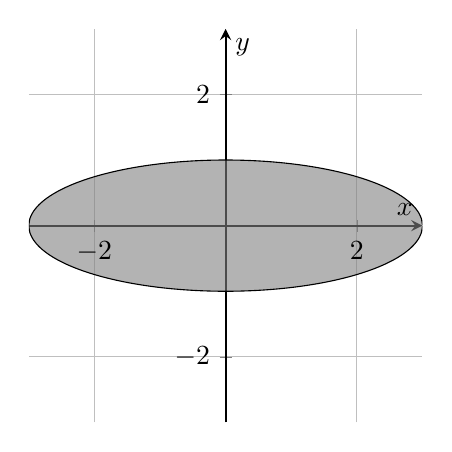
\begin{tikzpicture}
        \pgfplotsset{
            scale only axis,
        }
        \begin{axis}[
            xlabel=$x$,
            ylabel=$y$,
            width=5cm,
            height=5cm,
            axis lines=center,
            axis line style=thick, 
            xmin=-3,
            xmax=3,
            ymin=-3,
            ymax=3,
            grid=major,
            % ytick={50, 60, 62, 64, 66, 68, 70, 80, 90}
        ]
            % \label{test}
            % \addplot[mark=none, blue, domain=0:100]{0.236236236 * x + 65.43636363636364};
            
            \addplot [smooth, black, mark=none, domain=-3:3, samples=400, name path=A] {sqrt(1-\x^2 / 9)};
            \addplot [smooth, black, mark=none, domain=-3:3, samples=400, name path=B] {-sqrt(1-\x^2 / 9)};
            \addplot+ [gray, fill opacity=0.6] fill between [of=A and B, soft clip={domain=-3:3}];
        \end{axis}

        \end{tikzpicture}
    \end{center}

    \subsection*{18. }

    $\because f(x, y) = \sqrt y + \sqrt{25 - x^2 - y^2}$ is defined as 
    
    $$\left\{ \begin{array}{ll}  y \geq 0 \\ 25 - x^2 - y^2  \geq 0  \end{array}\right.$$

    $\therefore$ The domain of $f$ is $$\{ (x, y) | x^2 + y^2 \leq 25 \textrm{ and } y \geq 0 \}$$

    and the graph of $D(f)$ is illustrated below.

    \begin{center}
        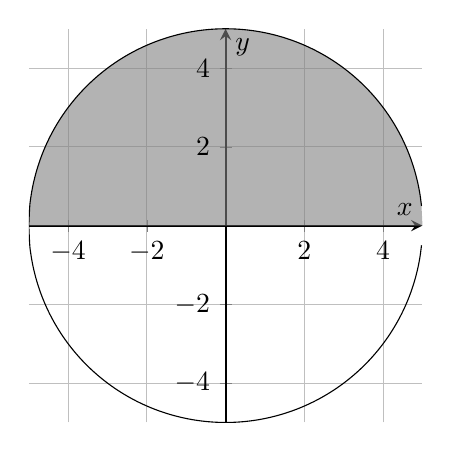
\begin{tikzpicture}
        \pgfplotsset{
            scale only axis,
        }
        \begin{axis}[
            xlabel=$x$,
            ylabel=$y$,
            width=5cm,
            height=5cm,
            axis lines=center,
            axis line style=thick, 
            xmin=-5,
            xmax=5,
            ymin=-5,
            ymax=5,
            grid=major,
            % ytick={50, 60, 62, 64, 66, 68, 70, 80, 90}
        ]
            % \label{test}
            % \addplot[mark=none, blue, domain=0:100]{0.236236236 * x + 65.43636363636364};
            
            \addplot [smooth, black, mark=none, domain=-5:5, samples=400, name path=A] {sqrt(25-\x^2)};
            \addplot [smooth, black, mark=none, domain=-5:5, samples=400, name path=B] {-sqrt(25-\x^2)};
            \addplot [draw=none, name path=C] {0};
            \addplot+ [gray, fill opacity=0.6] fill between [of=A and C, soft clip={domain=-5:5}];
        \end{axis}

        \end{tikzpicture}
    \end{center}

    \subsection*{20. }

    $\because f(x, y) = \arcsin(x^2 + y^2 - 2)$ is defined as $$-1 \leq x^2 + y^2 - 2 \leq 1$$

    $\therefore$ The domain of $f$ is $$\{ (x, y) | 1 \leq x^2 + y^2 \leq 3 \}$$

    and the graph of $D(f)$ is illustrated below.

    \begin{center}
        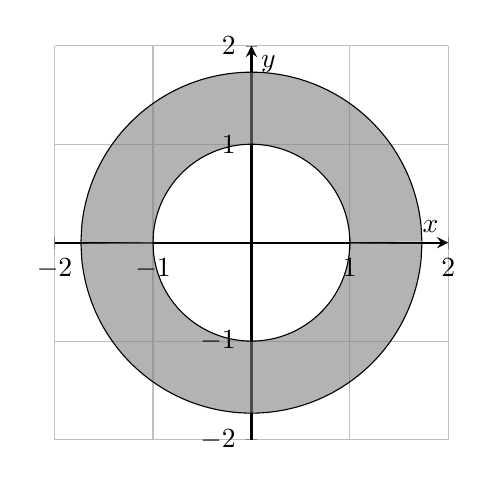
\begin{tikzpicture}
        \pgfplotsset{
            scale only axis,
        }
        \begin{axis}[
            xlabel=$x$,
            ylabel=$y$,
            width=5cm,
            height=5cm,
            axis lines=center,
            axis line style=thick, 
            xmin=-2,
            xmax=2,
            ymin=-2,
            ymax=2,
            grid=major,
            % ytick={50, 60, 62, 64, 66, 68, 70, 80, 90}
        ]
            % \label{test}
            % \addplot[mark=none, blue, domain=0:100]{0.236236236 * x + 65.43636363636364};
            
            \addplot [smooth, black, mark=none, domain=-sqrt(3):sqrt(3), samples=400, name path=A] {sqrt(3-\x^2)};
            \addplot [smooth, black, mark=none, domain=-sqrt(3):sqrt(3), samples=400, name path=B] {-sqrt(3-\x^2)};
            \addplot [smooth, black, mark=none, domain=-1:1, samples=400, name path=C] {sqrt(1-\x^2)};
            \addplot [smooth, black, mark=none, domain=-1:1, samples=400, name path=D] {-sqrt(1-\x^2)};
            \addplot+ [gray, fill opacity=0.6] fill between [of=A and C, soft clip={domain=-2:2}];
            \addplot+ [gray, fill opacity=0.6] fill between [of=B and D, soft clip={domain=-2:2}];
        \end{axis}

        \end{tikzpicture}
    \end{center}

    \subsection*{21. }

    $\because f(x, y, z) = \sqrt{1 - x^2 - y^2 - z^2}$ is defined when $$1 - x^2 - y^2 - z^2 \geq 0$$

    $\therefore$ The domain of $f$ is $$\{  (x, y, z) | x^2 + y^2 + z^2 \leq 1 \}$$

    and the graph of $D(f)$ is illustrated below.

    \begin{center}
        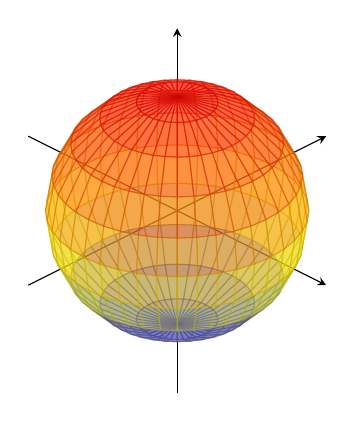
\begin{tikzpicture}
            \begin{axis}[%
                axis equal,
                width=10cm,
                height=10cm,
                axis lines = center,
                ticks=none,
                enlargelimits=0.3,
                view/h=45,
                scale uniformly strategy=units only,
            ]
            \addplot3[%
                opacity = 0.5,
                surf,
                z buffer = sort,
                samples = 21,
                variable = \u,
                variable y = \v,
                domain = 0:180,
                y domain = 0:360,
            ]
            ({cos(u)*sin(v)}, {sin(u)*sin(v)}, {cos(v)});
            \end{axis}
        \end{tikzpicture}
    \end{center}
    
\end{document}